%jen: repeats words in the bcakground section Tactile maps are not new to the cartographic record. Their value in facilitating orientation and navigation for the low vision and blind communities has been well established. However, their scope and availability has been greatly limited in the past by high production costs and limited interest from fields traditionally invested in map making and design. 

% same These maps have been designed as tools that enhance spatial understanding for people within a large range of visual capacities.  They abstract nonvisual cues from the pedestrian environment and consider circumstances that influence a full spectrum of experience. 

\subsubsection{Background and State of the Art}

\begin{comment}
I believe this is used somewhere else. Need to pull in.

Independent navigation is essential for autonomy and community participation in urban centers. 
Navigation solutions for both sighted and blind individuals fall into two important categories -- turn by turn directions, and maps. 
A common solution for Blind navigators is GPS programs that provide turn by turn directions. We tested the three blindness-aware GPS navigation mobile apps recommended by the American Foundation for the Blind: "Nearby Explorer", "The Seeing Eye GPS App", and "BlindSquare", and none offered a simultaneously sparse and informative solutions when used in conjunction with a portable Braille reader \cite{AFBBlindnessNavApps}, often because it is difficult to consume a lot of information portably with Braille readers on the go, and not all the information was equally relevant. 

\end{comment}


\subsubsection{Previous Development}
\label{sec:prev-devel-access}
The Taskar Center has two other relevant projects aiming to improve access to mobility and transportation for individuals with disabilities. The Taskar Center's overarching goal is 
to develop seamless regular-commute transportation customized assistance system that integrates multiple sources of current and critically relevant travel information.

This project build on AccessMaps, which itself depends on data from OpenSidewalks. As we will show, \jm{key points for extending accessmaps}




AccessMaps is \jm{Anat fill in introduction}.
Figure~\ref{fig:accessmap} shows the current version of the system in use. 

\begin{figure}
    \centering
    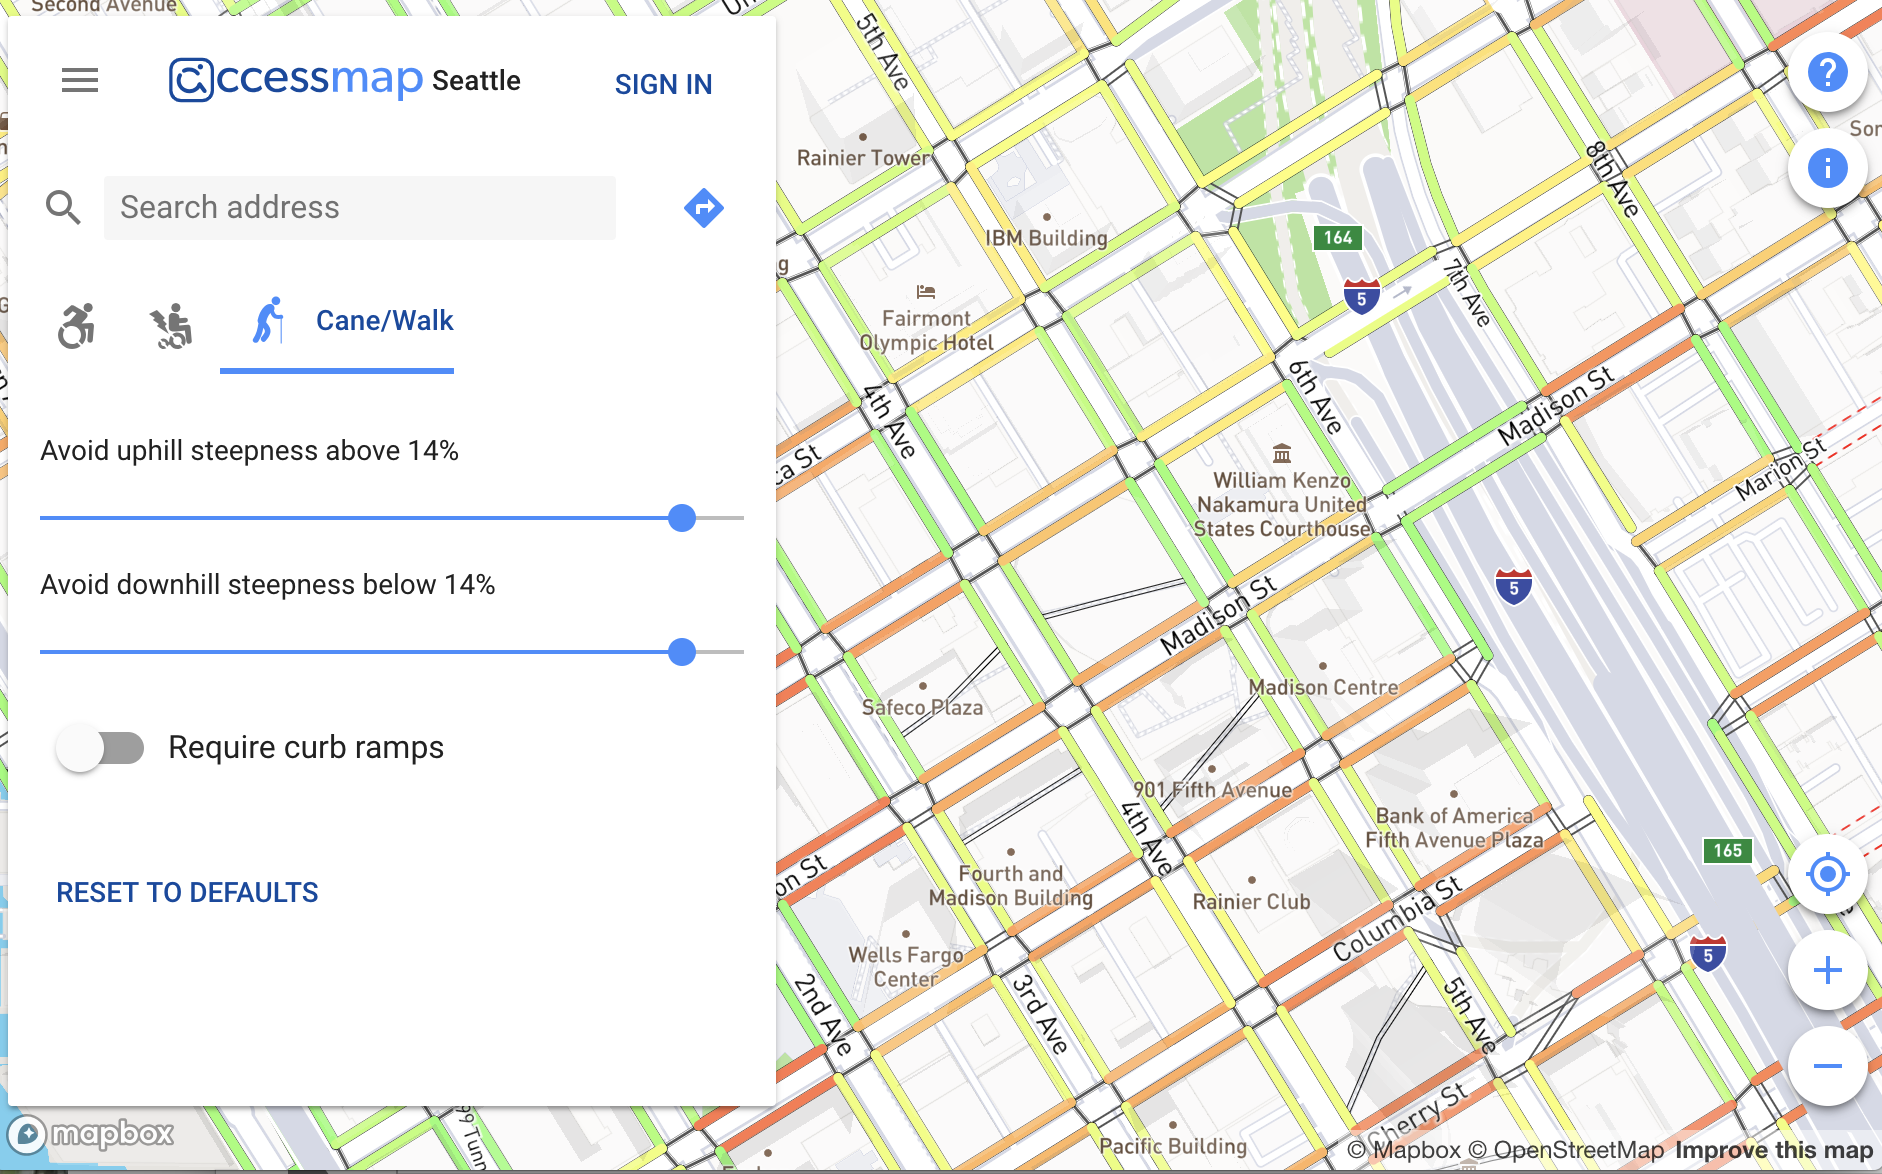
\includegraphics[width=5in]{pics/accessmap.png}
    \caption{AccessMap Screen Shot}
    \label{fig:accessmap}
\end{figure}

AccessMap currently can produce parametrically designed maps that always show the most up to data open data (derived from OpenSidewalks) about a region. 

\subsubsection{Proposed Development}

Operating hand-in-hand with AccessMap and OpenSidewalks (two projects discussed below), the goal of our work is to extend AccessMap to support users to automatically generate a custom 3D map model of any given area.  That model could then be printed at home, brought to a local library, or sent to a 3D printing service for relatively quick and inexpensive map production.  Beyond customizable map locations, ultimately the application would allow users to specify different scales and map features that are important to them.  

We will base our tactile design features on the comprehensive set of tactile map graphic symbols adopted by Braille Authority of North America (BANA) as created by (\cite{lobben2012tactile}, p. 107).% integrated into data driven design development tools and made available and consumable to landscape architects

%Anat: I commented this text out because I don't think it is product focused enough for NIDILLR's FIP in development. 
%The Tactile Maptile project designed the set of associated atomic symbols for that critical information.  Not only does this have implications for the map tiles specific to this project, but also more broadly works towards elevating pedestrian infrastructures in the context of our digital landscape.  This is important from a navigational perspective, but is also a reflection of the information designers, planners, and policy makers depend on to make significant decisions that affect our urban fabric.  Informed decisions based on incomplete data are not only difficult but also more prone to error and bias.  As we move rapidly towards sensor laced smart cities, it is critical these gaps be identified and understood in order to account for this influence on design and decision-making.  As such, this work is meant to take an accessible approach to data as it relates to pedestrian design and experience.

%Illustrative documentation of both the process and analysis that went into making these maps is directed more squarely at the design community. This project re-examines the pedestrian environment, with a focus on the specific needs of the low vision and blind communities. The goal of this work is to persuade designers to consider a broader spectrum of experience, and engage more critically in what it means to be designing inclusive cities.  

%This project is meant to bring attention to the deficiencies of the system currently place, in which accessibility checklists too often are accepted in lieu of truly inclusive design.  The straightforward approach is intended to remind designers that accessible design is good design, and if we want to build more equitable cities that means there is a huge spectrum of experiences we must first understand. 

\subsubsection{Validation}

\jm{ All studies need the following subsections to conform to the RFP:
\paragraph{Sample}
\paragraph{Environment}
\paragraph{Test Trials}
}

\ac{ needs writing


Our solution combines simple accessible interfaces with complex data integration and smart routing. To our users, the entire solution will be seamlessly presented in a workflow through which the travelers access a website, select the area of travel, the type of travel they wish to undertake in the area and travel preferences. The travelers are given the opportunity to verify the map location and features \textit{via} non-visual text-based exchange before printing the map.
% means what? A: means that in our UI pilot we found one of hardest things with building this UX/UI is ensuring that the tactile map model they got isn't of [Paris, Texas] when they actually meant [Paris, France]

The entire exchange is enabled and specifically designed for a portable 14-cell Braille-display. At the end, the traveler receives access to a downloadable 3D model file, access to an online URL where the model can be accessed for a specified duration, the option to have the model printed and sent to the user for a fee, and the option to subscribe to email alerts regarding any changes to the mapped region in the digital map repositories. 

}
